\documentclass[15pt]{article}
\usepackage[top=1in, bottom=1in, left=1in, right=1in]{geometry}
\usepackage[utf8]{inputenc}
\usepackage[T1]{fontenc}
\usepackage{amsmath}
\usepackage{amssymb}
\usepackage{lmodern}
\usepackage{bm}
\usepackage{scrextend}
%\usepackage{showframe}
\usepackage{calc}
\usepackage{changepage}
\usepackage{mdframed}
\usepackage{dsfont}
\usepackage{enumitem}
\usepackage{pbox}
\usepackage{setspace}
\usepackage{stmaryrd}
\usepackage{setspace}
\usepackage[table]{xcolor}
\usepackage{multicol}
\usepackage{mathtools}
\usepackage{hanging}
\usepackage{longtable}
\usepackage{aligned-overset}
\usepackage{ntheorem}
\usepackage{mdframed}
\usepackage[theorems,breakable]{tcolorbox}%
\usepackage{tikz}
\usetikzlibrary{positioning, arrows.meta}


\allowdisplaybreaks
\hbadness=10000
\makeatletter
\renewcommand*\env@matrix[1][*\c@MaxMatrixCols c]{%
  \hskip -\arraycolsep
  \let\@ifnextchar\new@ifnextchar
  \array{#1}}

\newcommand{\mathleft}{\@fleqntrue\@mathmargin10pt}
\newcommand{\mathcenter}{\@fleqnfalse}
\makeatother

\newcommand*{\QED}{\hfill\ensuremath{\square}} 
\newcommand{\R}{\mathbb{R}}
\newcommand{\N}{\mathbb{N}}
\newcommand{\Z}{\mathbb{Z}}
\newcommand{\Q}{\mathbb{Q}}
\newcommand{\p}{\mathcal{P}}
\newcommand{\K}{\mathbb{K}}
\newcommand{\C}{\mathbb{C}}
\newcommand{\la}{\langle}
\newcommand{\ra}{\rangle}


\newcommand{\bol}[1]{\mathbf{#1}}


\newlength{\hangwidth}
\newcommand{\newhang}[1]{\settowidth{\hangwidth}{#1}\par\hangpara{\hangwidth}{1}#1}

\newcommand{\norm}[1]{\lVert #1 \rVert}

\def\Abstand{1cm}

\newtcbtheorem{lemma}{Lemma}{%
        theorem name,%
        colframe=gray,%
        fonttitle=\bfseries,
        boxsep=5pt,
        left=5pt, right=5pt, top=5pt, bottom=5pt
    }{lem}

\newtcbtheorem{theorem}{Theorem}{
        theorem name,%
        colframe=gray,%
        fonttitle=\bfseries,
        boxsep=5pt,
        left=5pt, right=5pt, top=5pt, bottom=5pt
    }{thm}

\newtcbtheorem{definition}{Definition}{
      theorem name,%
      colframe=gray,%
      fonttitle=\bfseries,
      boxsep=5pt,
      left=5pt, right=5pt, top=5pt, bottom=5pt
  }{def}

\title{Notes on Physics Informed Diffusion Models}
\author{ }
\date{}


\begin{document}


\maketitle

\newlength\breite
\setlength\breite{\linewidth-4pt}
\setlength\fboxsep{0pt}
\setlength\fboxrule{0.25pt}
\setlength{\abovedisplayskip}{3mm} %Abstand OBEN zw. Text und Formel
\setlength{\belowdisplayskip}{3mm} %Abstand OBEN zw. Text und Formel
\setlength\itemsep{0pt}
\setlength\parindent{0pt}


\mathleft

\section*{Preliminaries}

\begin{figure}[h]
\centering
\resizebox{\linewidth}{!}{%
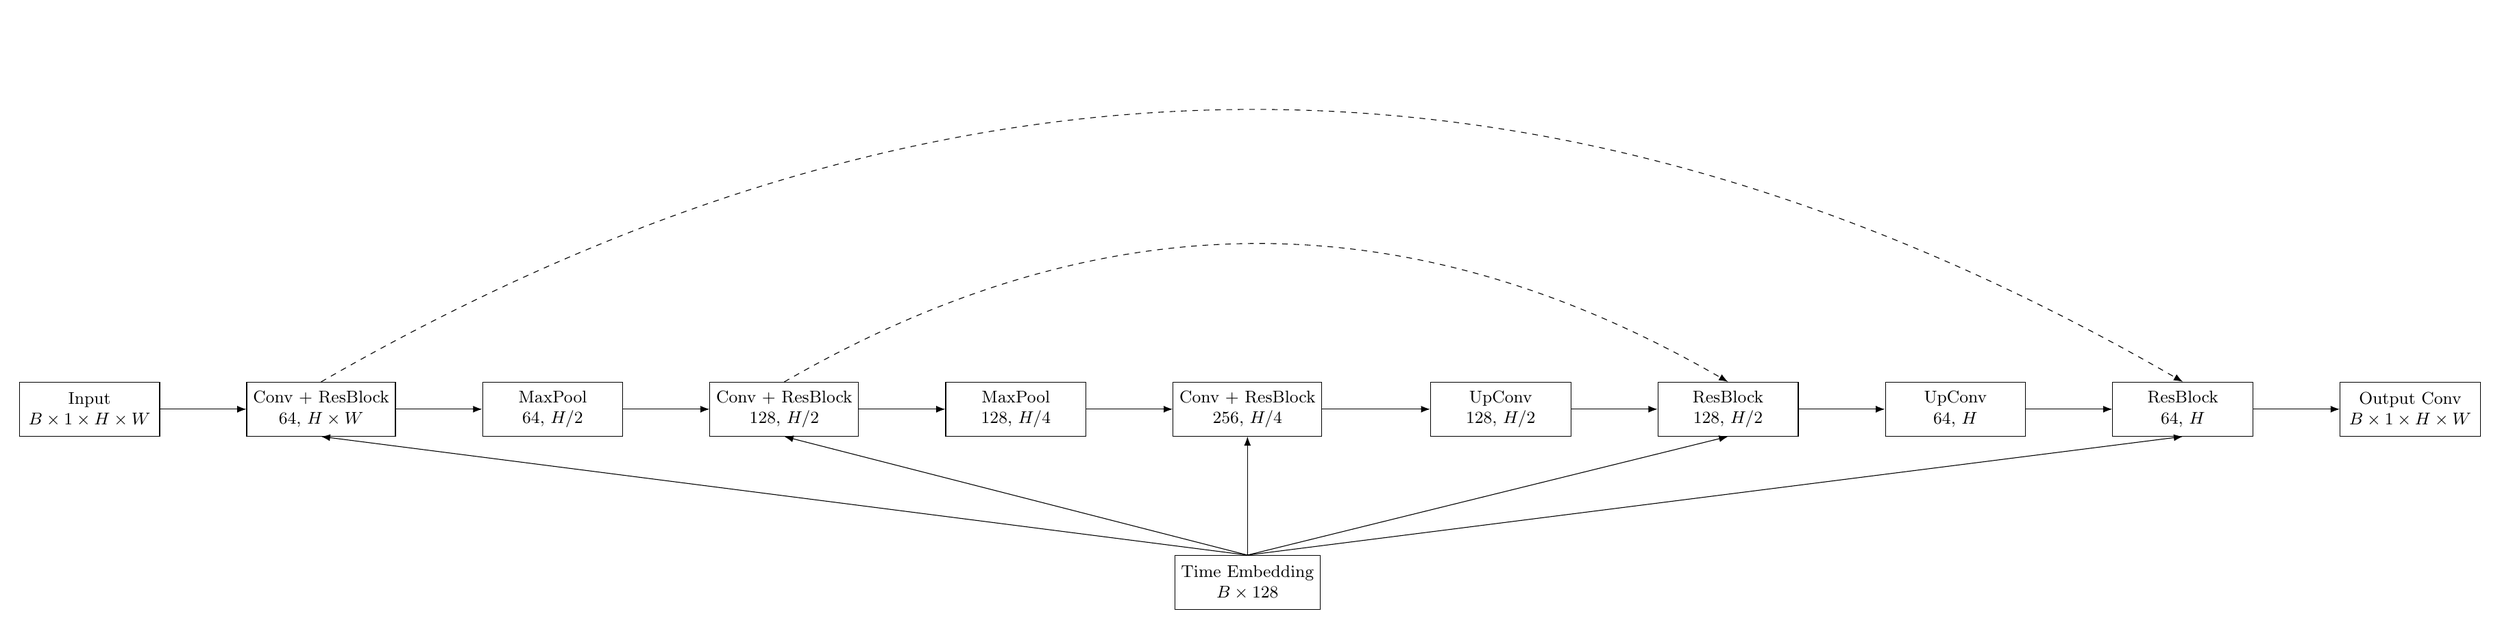
\begin{tikzpicture}[
    block/.style={
        draw,
        rectangle,
        minimum height=1cm,
        minimum width=2.6cm,
        align=center,
        font=\small
    },
    skip/.style={draw, dashed, -{Latex}},
    arrow/.style={-{Latex}}
]

% Encoder
\node[block] (input) {Input\\$B\times1\times H\times W$};

\node[block, right=1.6cm of input] (enc1) {Conv + ResBlock\\$64,\, H\times W$};

\node[block, right=1.6cm of enc1] (pool1) {MaxPool\\$64,\, H/2$};

\node[block, right=1.6cm of pool1] (enc2) {Conv + ResBlock\\$128,\, H/2$};

\node[block, right=1.6cm of enc2] (pool2) {MaxPool\\$128,\, H/4$};

\node[block, right=1.6cm of pool2] (bottleneck) {Conv + ResBlock\\$256,\, H/4$};

% Decoder
\node[block, right=2.0cm of bottleneck] (up2) {UpConv\\$128,\, H/2$};

\node[block, right=1.6cm of up2] (dec2) {ResBlock\\$128,\, H/2$};

\node[block, right=1.6cm of dec2] (up1) {UpConv\\$64,\, H$};

\node[block, right=1.6cm of up1] (dec1) {ResBlock\\$64,\, H$};

\node[block, right=1.6cm of dec1] (output) {Output Conv\\$B\times1\times H\times W$};

% Main arrows
\draw[arrow] (input) -- (enc1);
\draw[arrow] (enc1) -- (pool1);
\draw[arrow] (pool1) -- (enc2);
\draw[arrow] (enc2) -- (pool2);
\draw[arrow] (pool2) -- (bottleneck);
\draw[arrow] (bottleneck) -- (up2);
\draw[arrow] (up2) -- (dec2);
\draw[arrow] (dec2) -- (up1);
\draw[arrow] (up1) -- (dec1);
\draw[arrow] (dec1) -- (output);

% Skip connections
\draw[skip] (enc1.north) to[bend left=30] (dec1.north);
\draw[skip] (enc2.north) to[bend left=30] (dec2.north);

% Time embedding
\node[block, below=2.2cm of bottleneck] (time) {Time Embedding\\$B\times128$};

\draw[arrow] (time.north) -- (enc1.south);
\draw[arrow] (time.north) -- (enc2.south);
\draw[arrow] (time.north) -- (bottleneck.south);
\draw[arrow] (time.north) -- (dec2.south);
\draw[arrow] (time.north) -- (dec1.south);

\end{tikzpicture}
}
\caption{Time-conditioned UNet architecture used in the diffusion model.}
\end{figure}


\end{document}


